
%% bare_conf.tex
%% V1.3
%% 2007/01/11
%% by Michael Shell
%% See:
%% http://www.michaelshell.org/
%% for current contact information.
%%
%% This is a skeleton file demonstrating the use of IEEEtran.cls
%% (requires IEEEtran.cls version 1.7 or later) with an IEEE conference paper.
%%
%% Support sites:
%% http://www.michaelshell.org/tex/ieeetran/
%% http://www.ctan.org/tex-archive/macros/latex/contrib/IEEEtran/
%% and
%% http://www.ieee.org/

%%*************************************************************************
%% Legal Notice:
%% This code is offered as-is without any warranty either expressed or
%% implied; without even the implied warranty of MERCHANTABILITY or
%% FITNESS FOR A PARTICULAR PURPOSE! 
%% User assumes all risk.
%% In no event shall IEEE or any contributor to this code be liable for
%% any damages or losses, including, but not limited to, incidental,
%% consequential, or any other damages, resulting from the use or misuse
%% of any information contained here.
%%
%% All comments are the opinions of their respective authors and are not
%% necessarily endorsed by the IEEE.
%%
%% This work is distributed under the LaTeX Project Public License (LPPL)
%% ( http://www.latex-project.org/ ) version 1.3, and may be freely used,
%% distributed and modified. A copy of the LPPL, version 1.3, is included
%% in the base LaTeX documentation of all distributions of LaTeX released
%% 2003/12/01 or later.
%% Retain all contribution notices and credits.
%% ** Modified files should be clearly indicated as such, including  **
%% ** renaming them and changing author support contact information. **
%%
%% File list of work: IEEEtran.cls, IEEEtran_HOWTO.pdf, bare_adv.tex,
%%                    bare_conf.tex, bare_jrnl.tex, bare_jrnl_compsoc.tex
%%*************************************************************************

% *** Authors should verify (and, if needed, correct) their LaTeX system  ***
% *** with the testflow diagnostic prior to trusting their LaTeX platform ***
% *** with production work. IEEE's font choices can trigger bugs that do  ***
% *** not appear when using other class files.                            ***
% The testflow support page is at:
% http://www.michaelshell.org/tex/testflow/

% Note that the a4paper option is mainly intended so that authors in
% countries using A4 can easily print to A4 and see how their papers will
% look in print - the typesetting of the document will not typically be
% affected with changes in paper size (but the bottom and side margins will).
% Use the testflow package mentioned above to verify correct handling of
% both paper sizes by the user's LaTeX system.
%
% Also note that the "draftcls" or "draftclsnofoot", not "draft", option
% should be used if it is desired that the figures are to be displayed in
% draft mode.
%
\documentclass[conference]{IEEEtran}
% Add the compsoc option for Computer Society conferences.
%
% If IEEEtran.cls has not been installed into the LaTeX system files,
% manually specify the path to it like:
% \documentclass[conference]{../sty/IEEEtran}





% Some very useful LaTeX packages include:
% (uncomment the ones you want to load)
\usepackage{graphicx}
\usepackage{listings}


% *** MISC UTILITY PACKAGES ***
%
%\usepackage{ifpdf}
% Heiko Oberdiek's ifpdf.sty is very useful if you need conditional
% compilation based on whether the output is pdf or dvi.
% usage:
% \ifpdf
%   % pdf code
% \else
%   % dvi code
% \fi
% The latest version of ifpdf.sty can be obtained from:
% http://www.ctan.org/tex-archive/macros/latex/contrib/oberdiek/
% Also, note that IEEEtran.cls V1.7 and later provides a builtin
% \ifCLASSINFOpdf conditional that works the same way.
% When switching from latex to pdflatex and vice-versa, the compiler may
% have to be run twice to clear warning/error messages.






% *** CITATION PACKAGES ***
%
%\usepackage{cite}
% cite.sty was written by Donald Arseneau
% V1.6 and later of IEEEtran pre-defines the format of the cite.sty package
% \cite{} output to follow that of IEEE. Loading the cite package will
% result in citation numbers being automatically sorted and properly
% "compressed/ranged". e.g., [1], [9], [2], [7], [5], [6] without using
% cite.sty will become [1], [2], [5]--[7], [9] using cite.sty. cite.sty's
% \cite will automatically add leading space, if needed. Use cite.sty's
% noadjust option (cite.sty V3.8 and later) if you want to turn this off.
% cite.sty is already installed on most LaTeX systems. Be sure and use
% version 4.0 (2003-05-27) and later if using hyperref.sty. cite.sty does
% not currently provide for hyperlinked citations.
% The latest version can be obtained at:
% http://www.ctan.org/tex-archive/macros/latex/contrib/cite/
% The documentation is contained in the cite.sty file itself.






% *** GRAPHICS RELATED PACKAGES ***
%
\ifCLASSINFOpdf
  % \usepackage[pdftex]{graphicx}
  % declare the path(s) where your graphic files are
  % \graphicspath{{../pdf/}{../jpeg/}}
  % and their extensions so you won't have to specify these with
  % every instance of \includegraphics
  % \DeclareGraphicsExtensions{.pdf,.jpeg,.png}
\else
  % or other class option (dvipsone, dvipdf, if not using dvips). graphicx
  % will default to the driver specified in the system graphics.cfg if no
  % driver is specified.
  % \usepackage[dvips]{graphicx}
  % declare the path(s) where your graphic files are
  % \graphicspath{{../eps/}}
  % and their extensions so you won't have to specify these with
  % every instance of \includegraphics
  % \DeclareGraphicsExtensions{.eps}
\fi
% graphicx was written by David Carlisle and Sebastian Rahtz. It is
% required if you want graphics, photos, etc. graphicx.sty is already
% installed on most LaTeX systems. The latest version and documentation can
% be obtained at: 
% http://www.ctan.org/tex-archive/macros/latex/required/graphics/
% Another good source of documentation is "Using Imported Graphics in
% LaTeX2e" by Keith Reckdahl which can be found as epslatex.ps or
% epslatex.pdf at: http://www.ctan.org/tex-archive/info/
%
% latex, and pdflatex in dvi mode, support graphics in encapsulated
% postscript (.eps) format. pdflatex in pdf mode supports graphics
% in .pdf, .jpeg, .png and .mps (metapost) formats. Users should ensure
% that all non-photo figures use a vector format (.eps, .pdf, .mps) and
% not a bitmapped formats (.jpeg, .png). IEEE frowns on bitmapped formats
% which can result in "jaggedy"/blurry rendering of lines and letters as
% well as large increases in file sizes.
%
% You can find documentation about the pdfTeX application at:
% http://www.tug.org/applications/pdftex





% *** MATH PACKAGES ***
%
%\usepackage[cmex10]{amsmath}
% A popular package from the American Mathematical Society that provides
% many useful and powerful commands for dealing with mathematics. If using
% it, be sure to load this package with the cmex10 option to ensure that
% only type 1 fonts will utilized at all point sizes. Without this option,
% it is possible that some math symbols, particularly those within
% footnotes, will be rendered in bitmap form which will result in a
% document that can not be IEEE Xplore compliant!
%
% Also, note that the amsmath package sets \interdisplaylinepenalty to 10000
% thus preventing page breaks from occurring within multiline equations. Use:
%\interdisplaylinepenalty=2500
% after loading amsmath to restore such page breaks as IEEEtran.cls normally
% does. amsmath.sty is already installed on most LaTeX systems. The latest
% version and documentation can be obtained at:
% http://www.ctan.org/tex-archive/macros/latex/required/amslatex/math/

\usepackage{mathtools}



% *** SPECIALIZED LIST PACKAGES ***
%
%\usepackage{algorithmic}
% algorithmic.sty was written by Peter Williams and Rogerio Brito.
% This package provides an algorithmic environment fo describing algorithms.
% You can use the algorithmic environment in-text or within a figure
% environment to provide for a floating algorithm. Do NOT use the algorithm
% floating environment provided by algorithm.sty (by the same authors) or
% algorithm2e.sty (by Christophe Fiorio) as IEEE does not use dedicated
% algorithm float types and packages that provide these will not provide
% correct IEEE style captions. The latest version and documentation of
% algorithmic.sty can be obtained at:
% http://www.ctan.org/tex-archive/macros/latex/contrib/algorithms/
% There is also a support site at:
% http://algorithms.berlios.de/index.html
% Also of interest may be the (relatively newer and more customizable)
% algorithmicx.sty package by Szasz Janos:
% http://www.ctan.org/tex-archive/macros/latex/contrib/algorithmicx/




% *** ALIGNMENT PACKAGES ***
%
%\usepackage{array}
% Frank Mittelbach's and David Carlisle's array.sty patches and improves
% the standard LaTeX2e array and tabular environments to provide better
% appearance and additional user controls. As the default LaTeX2e table
% generation code is lacking to the point of almost being broken with
% respect to the quality of the end results, all users are strongly
% advised to use an enhanced (at the very least that provided by array.sty)
% set of table tools. array.sty is already installed on most systems. The
% latest version and documentation can be obtained at:
% http://www.ctan.org/tex-archive/macros/latex/required/tools/


%\usepackage{mdwmath}
%\usepackage{mdwtab}
% Also highly recommended is Mark Wooding's extremely powerful MDW tools,
% especially mdwmath.sty and mdwtab.sty which are used to format equations
% and tables, respectively. The MDWtools set is already installed on most
% LaTeX systems. The lastest version and documentation is available at:
% http://www.ctan.org/tex-archive/macros/latex/contrib/mdwtools/


% IEEEtran contains the IEEEeqnarray family of commands that can be used to
% generate multiline equations as well as matrices, tables, etc., of high
% quality.


%\usepackage{eqparbox}
% Also of notable interest is Scott Pakin's eqparbox package for creating
% (automatically sized) equal width boxes - aka "natural width parboxes".
% Available at:
% http://www.ctan.org/tex-archive/macros/latex/contrib/eqparbox/





% *** SUBFIGURE PACKAGES ***
%\usepackage[tight,footnotesize]{subfigure}
% subfigure.sty was written by Steven Douglas Cochran. This package makes it
% easy to put subfigures in your figures. e.g., "Figure 1a and 1b". For IEEE
% work, it is a good idea to load it with the tight package option to reduce
% the amount of white space around the subfigures. subfigure.sty is already
% installed on most LaTeX systems. The latest version and documentation can
% be obtained at:
% http://www.ctan.org/tex-archive/obsolete/macros/latex/contrib/subfigure/
% subfigure.sty has been superceeded by subfig.sty.



%\usepackage[caption=false]{caption}
%\usepackage[font=footnotesize]{subfig}
% subfig.sty, also written by Steven Douglas Cochran, is the modern
% replacement for subfigure.sty. However, subfig.sty requires and
% automatically loads Axel Sommerfeldt's caption.sty which will override
% IEEEtran.cls handling of captions and this will result in nonIEEE style
% figure/table captions. To prevent this problem, be sure and preload
% caption.sty with its "caption=false" package option. This is will preserve
% IEEEtran.cls handing of captions. Version 1.3 (2005/06/28) and later 
% (recommended due to many improvements over 1.2) of subfig.sty supports
% the caption=false option directly:
%\usepackage[caption=false,font=footnotesize]{subfig}
%
% The latest version and documentation can be obtained at:
% http://www.ctan.org/tex-archive/macros/latex/contrib/subfig/
% The latest version and documentation of caption.sty can be obtained at:
% http://www.ctan.org/tex-archive/macros/latex/contrib/caption/




% *** FLOAT PACKAGES ***
%
%\usepackage{fixltx2e}
% fixltx2e, the successor to the earlier fix2col.sty, was written by
% Frank Mittelbach and David Carlisle. This package corrects a few problems
% in the LaTeX2e kernel, the most notable of which is that in current
% LaTeX2e releases, the ordering of single and double column floats is not
% guaranteed to be preserved. Thus, an unpatched LaTeX2e can allow a
% single column figure to be placed prior to an earlier double column
% figure. The latest version and documentation can be found at:
% http://www.ctan.org/tex-archive/macros/latex/base/



%\usepackage{stfloats}
% stfloats.sty was written by Sigitas Tolusis. This package gives LaTeX2e
% the ability to do double column floats at the bottom of the page as well
% as the top. (e.g., "\begin{figure*}[!b]" is not normally possible in
% LaTeX2e). It also provides a command:
%\fnbelowfloat
% to enable the placement of footnotes below bottom floats (the standard
% LaTeX2e kernel puts them above bottom floats). This is an invasive package
% which rewrites many portions of the LaTeX2e float routines. It may not work
% with other packages that modify the LaTeX2e float routines. The latest
% version and documentation can be obtained at:
% http://www.ctan.org/tex-archive/macros/latex/contrib/sttools/
% Documentation is contained in the stfloats.sty comments as well as in the
% presfull.pdf file. Do not use the stfloats baselinefloat ability as IEEE
% does not allow \baselineskip to stretch. Authors submitting work to the
% IEEE should note that IEEE rarely uses double column equations and
% that authors should try to avoid such use. Do not be tempted to use the
% cuted.sty or midfloat.sty packages (also by Sigitas Tolusis) as IEEE does
% not format its papers in such ways.





% *** PDF, URL AND HYPERLINK PACKAGES ***
%
%\usepackage{url}
% url.sty was written by Donald Arseneau. It provides better support for
% handling and breaking URLs. url.sty is already installed on most LaTeX
% systems. The latest version can be obtained at:
% http://www.ctan.org/tex-archive/macros/latex/contrib/misc/
% Read the url.sty source comments for usage information. Basically,
% \url{my_url_here}.





% *** Do not adjust lengths that control margins, column widths, etc. ***
% *** Do not use packages that alter fonts (such as pslatex).         ***
% There should be no need to do such things with IEEEtran.cls V1.6 and later.
% (Unless specifically asked to do so by the journal or conference you plan
% to submit to, of course. )


% correct bad hyphenation here
\hyphenation{op-tical net-works semi-conduc-tor}


\begin{document}
%
% paper title
% can use linebreaks \\ within to get better formatting as desired
\title{A GPU Solution for Signal Anomaly Detection in the Frequency Domain}


% author names and affiliations
% use a multiple column layout for up to three different
% affiliations
\author{
\IEEEauthorblockN{Nathan Jordan}
\IEEEauthorblockA{Department of Computer Science\\
University of Nevada, Reno\\
Reno, Nevada 89512\\
Email: njordan@cse.unr.edu}
\and
\IEEEauthorblockN{Lee Barford}
\IEEEauthorblockA{Agilent Technologies\\
Santa Clara, CA\\
Email: lee.barford@gmail.com}
\and
\IEEEauthorblockN{Fred Harris}
\IEEEauthorblockA{Department of Computer Science\\
University of Nevada, Reno\\
Reno, Nevada 89512\\
Email: fred.harris@cse.unr.edu
}
}

% conference papers do not typically use \thanks and this command
% is locked out in conference mode. If really needed, such as for
% the acknowledgment of grants, issue a \IEEEoverridecommandlockouts
% after \documentclass

% for over three affiliations, or if they all won't fit within the width
% of the page, use this alternative format:
% 
%\author{\IEEEauthorblockN{Michael Shell\IEEEauthorrefmark{1},
%Homer Simpson\IEEEauthorrefmark{2},
%James Kirk\IEEEauthorrefmark{3}, 
%Montgomery Scott\IEEEauthorrefmark{3} and
%Eldon Tyrell\IEEEauthorrefmark{4}}
%\IEEEauthorblockA{\IEEEauthorrefmark{1}School of Electrical and Computer Engineering\\
%Georgia Institute of Technology,
%Atlanta, Georgia 30332--0250\\ Email: see http://www.michaelshell.org/contact.html}
%\IEEEauthorblockA{\IEEEauthorrefmark{2}Twentieth Century Fox, Springfield, USA\\
%Email: homer@thesimpsons.com}
%\IEEEauthorblockA{\IEEEauthorrefmark{3}Starfleet Academy, San Francisco, California 96678-2391\\
%Telephone: (800) 555--1212, Fax: (888) 555--1212}
%\IEEEauthorblockA{\IEEEauthorrefmark{4}Tyrell Inc., 123 Replicant Street, Los Angeles, California 90210--4321}}




% use for special paper notices
%\IEEEspecialpapernotice{(Invited Paper)}




% make the title area
\maketitle


\begin{abstract}
%\boldmath


As the extensibility of GPU computing rapidly increases, we often find them useful
 for different applications in the field of science and engineering. Libraries
 written for engineering tasks such as CULA (Cuda Linear Algebra), CUFFT (Cuda 
 Fast Fourier Transform), and CUBLAS (Cuda Basic Linear Algebra Subprograms) have
 made it easier for programmers to achieve a significant performance increase when
 solving problems in the fields of engineering and math. In signal processing we can
 use the GPU to perform discrete Fourier transforms on time-domain signal strength
 to represent the data in the frequency domain. With the data in this format, we can 
 calculate signal strength of various frequencies very efficiently, and further determine
 if a transmission on a particular frequency has taken place. Speedups in excess of X\%
 were achievable using a GPU-based implementation utilizing the cuFFT library over a CPU
 implementation utilizing the most performance optimized CPU-based FFT library, FFTW.

\end{abstract}

\IEEEpeerreviewmaketitle

\section{Introduction}

The ubiquity and necessity of parallel computing has begun to show itself
in recent years, and companies have found the need to adapt their hardware to
facilitate parallelism. This is becoming a necessary change to allow for
speedups that historically would be delivered by an increase in CPU clock
frequency. NVIDIA, harnessing the inherent SIMD (single instruction multiple data)
properties of their GPU's, created the CUDA API, which allows programmers
to write C/C++ code that takes advantage of the hundreds or thousands of 
cores present on modern NVIDIA GPU's, without having to learn a new language,
or have intimate knowledge of the hardware. 

Consequently, many applications that were formerly bound by the lack of floating
point throughput of most CPU's can take advantage of the massive parallelism
that a GPU can provide. Applications ranging from scientific and engineering 
number crunching to sorting algorithms (which run many times faster than their
CPU counterparts \cite{x}). Even though the performance of everyday algorithms
can be improved by the GPU, the place where they most outperform the CPU is 
in applications which require large amounts of floating point arithmetic. 
Most scientific and engineering-related fields have large and computationally
difficult problems that need to be solved as fast as possible. In this paper,
we will look at a potential application of the GPU to solve problems in the
field of Electrical Engineering; more spefically signal analysis and processing.

If we are working with a radio signal, we can take the digitized signal and
use the GPU to detect anomalies in a particular frequency range. If we can
detect that a transmission has occurred on a known frequency, then we can
intercept that transmission (provided it is not encrpyted), or attempt
to triangulate the position of the signal using multiple antennas that
are synchronized to a certain degree. This paper presents a GPU algorithm
to perform this task significantly faster than a CPU using well-optimized
libraries.

The rest of this paper is organized as follows: first some of the background
information surrounding the topic will be covered; second, the sequential implementation
will be discussed; third, the parallel implementation, including pipelined and
non-pipelined versions, will be explained; finally, we will end the paper
with some concludatory remarks and the future direction of the project.
 
\hfill May 9th, 2013

\section{Background}

In engineering, the Fourier Transform is applicable to many topics such as 
differential equations, spectroscopy, and quantum mechanics. In electrical
engineering and signal processing, the Fourier transform can be used to
switch between the time and frequency domains. Information in the time
domain by itself it of little use when trying to infer information about
a signal, as it is a representation of many different bands of frequencies
superimposed on top of each other. If we perform a Fourier Transform on 
a signal represented in the time domain, the result is a frequency spectrum
that provides the resulting values in the complex plane. The frequency
spectrum can be used to see which frequencies have the greatest power
in a particular signal. If the signal we are analyzing is a radio wave
generated by an antenna, we can determine which frequencies are being
transmitted on, and quite possibly intercept the transmission as well.

There are several implementations of the Fourier Transform. The one most
commonly used by engineers in real applications is the FFT, or Fast
Fourier Transform. As one may suspect, the FFT gets its name from the
efficiency in which it computes the transform compared to other methods,
however despite its speed, it does not compromise accuracy. There are a 
few implementations of the FFT, the most common of which being the Cooley-
Turkey algorithm, and another being the Bluestein's algorithm, which is
used in some cases when the FFT size is near a prime number (where Cooley-
Turkey performs poorly). 

The FFTW library is one of the most popular FFT libraries in use in
open-source software. It is also unsurprisingly by far and away the fastest open-source
FFT library. Its only competition is Intel Math Kernel Library (MKL),
a proprietary software developed by Intel for the Intel Compiler. These
two FFT libraries are comparable in performance, with MKL usually outperforming
FFTW for larger FFT's. In this project, we will be using FFTW as our 
FFT library, due to its popularity, openness, and speed.

\begin{figure}[ht!]
\centering
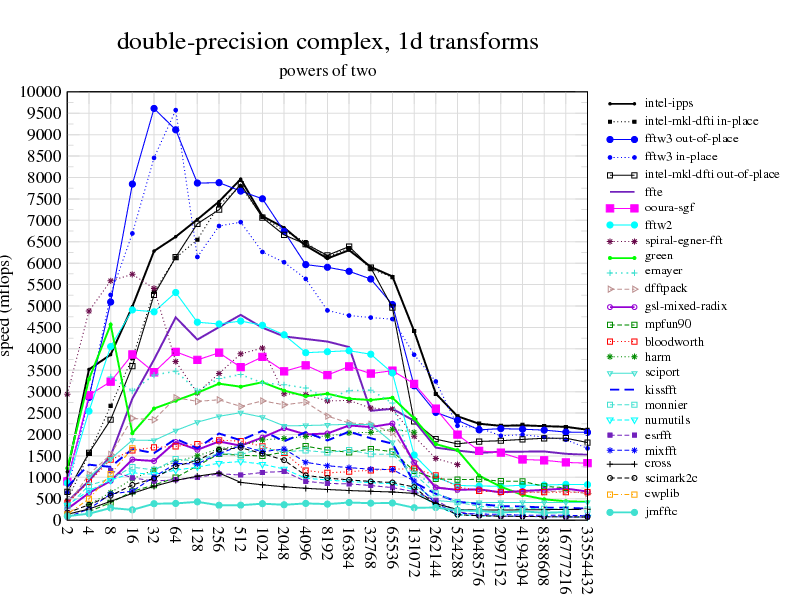
\includegraphics[width=3.5in]{fftwmkl.png}
\caption{Benchmarks comparing the performance of FFTW, MKL and other FFT libraries. FFTW and MKL are the fastest, shown in blue and black respectively. \cite{fftw:benchmarks}}
\label{fig:fftwmkl}
\end{figure}


\begin{figure}[ht!]
\centering
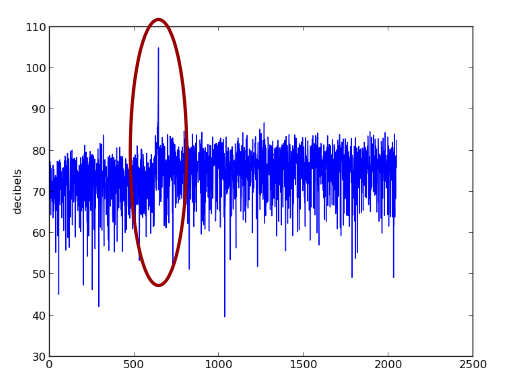
\includegraphics[width=3.5in]{signalgraph.png}
\caption{Following the FFT calculation and signal analysis, a transmission is clearly visible in the frequency domain}
\label{fig:pipeline}
\end{figure}

With the introduction of CUDA in 2008, NVIDIA has stepped into the
high-performance computing arena. Due to their inherently parallel
nature and fast floating point operations, GPU's handily lend themselves 
to many engineering problems. NVIDIA has created their own implementation
of the FFT, called cuFFT (CUDA FFT) for the convenience of programmers
writing engineering software. cuFFT is modeled after its CPU-based counterpart
FFTW, and implements its algorithms in a similar fashion. To speed up
the transition for programmers used to FFTW, NVIDIA made the API for
cuFFT almost identical to that of FFTW, making it easy to port existing
code to the GPU for a significant speedup. For the parallel implementation
of this project, cuFFT was used due to its similarity to FFTW for comparison
purposes, and more importantly,  to avoid implementing an FFT manually
on a GPU. 

\section{Sequential Implementation}

The sequential version of the program is relatively straightforward. Initially,
the input to the program is a binary flat file consisting of 8-bit integers 
representing the signal received by an antenna in the time domain. Each 8-bit
integer is converted to a single-precision floating point number, and added
to a vector for later processing. After the data is read from the file, arrays
are allocated for the FFT computation and the main algorithm begins. An FFT of size
4096 ($2^{12}$) was chosen as it exhibits the best performance when using FFTW and cuFFT.
A real-to-complex FFT is performed incrementally on the input signal information
and is stored in a result vector that contains both the real and complex portions
of the transform as a complex conjugate. After the FFT is calculated, the modulus 
of the complex result are calculated for each frequency bin to give us the
magnitude of the frequency, as seen in Equation \ref{eq:modulus}.

\begin{equation}
|z|=\sqrt{ x^2 + yi^2 } \label{eq:modulus}
\end{equation}

Once we have the magnitude of each of the frequency bins calculated by the FFT,
we can put them into the logarithmic decibel (dB) scale by using the formula 
described by equation \ref{eq:dB}.

\begin{equation}
Z=20 \times \log_{10}(|z|) \label{eq:dB}
\end{equation}

After this calculation there are two different approaches we can take. The first,
which is much simpler, compares the computed signal strength to a constant value
set before runtime. If the signal strength for a particular frequency bin exceeds
this value, we assume that a transmission has begun on that particular frequency.
We can filter out some noise by applying another constant value that is the 
amount of time that the signal strength for a particular bin must exceed the 
signal strength constant in order to classify it as a transmission instead of 
random noise.
Given the unsophisticated nature of this method, it is unsurprising that it is not
the most most reliable method to determine a legitimate transmission.

\begin{figure}[ht!]
\centering
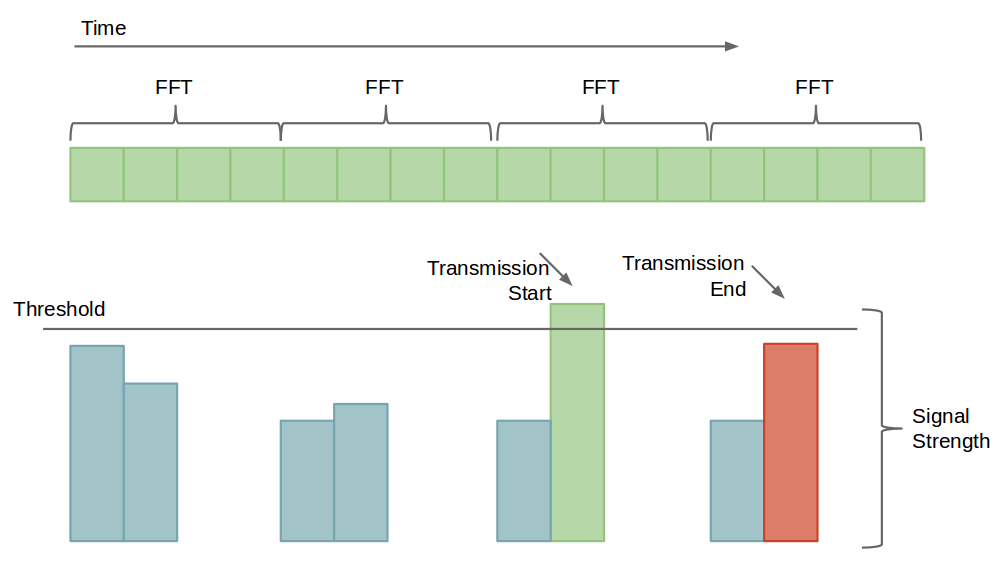
\includegraphics[width=3.5in]{sequentialgraphic.png}
\caption{A graphic showing the how the sequential program runs.}
\label{fig:pipeline}
\end{figure}

A second approach is to dynamically modify these values as the signal strengths
are computed during runtime. This allows for the level of noise to change during
the transmission, and can be used as a more reliable method to distinguish between
noise and actual transmissions. This increased accuracy comes at the cost of
additional computational overhead during the execution of the algorithm.

Once a transmission is detected, a new entry for it is created in a transmission log vector
containing its frequency, maximum strength, and start time. Also during each iteration,
the algorithm will then check to see if a current transmission's strength level
has fallen below the threshold value. If this is the case, its end time will
be added to the transmission log. Any subsequent rise of that frequency over the
threshold value will trigger the creation of a new transmission log.

Once the algorithm has been completed, the transmission log is written to a file
of the users choosing for further analysis.

\section{Parallel Implementation}

With the parallel implementation, we use an algorithmically-similar approach 
to our sequential implementation. Like the sequential version, we will be calculating
the FFT of our input signal information to transform it to the frequency domain
and calculating the complex modulus of the result. Unlike the CPU implementation,
however, the signal information is not directly available to the card, and must
be copied across the PCI Express (PCIE) bus. The PCIE bus is orders of magnitude
slower than any kind of operation performed on a GPU or CPU, including memory
accesses. As such, the PCIE bus often becomes a performance bottleneck for
GPU programs, especially when the amount of data to be transferred is quite large.

To solve this, we can use a technique called pipelining, which allows us to
minimize this bottleneck. Pipelining, which is similar to the instruction
pipeline used in the CPU, breaks memory transfer and computation of data into different
parts that can be performed independently of each other. Blocks of data are transferred
one at a time across the PCIE bus and are computed on once they arrive on the GPU.
This way, we can start computing the FFTs and signal analysis right away without
having to wait for the entire chunk of data to be transferred across the PCIE
bus. For this paper, a non-pipelined approach will be implemented first for
comparison purposes, and a pipelined version will follow.

\begin{figure}[ht!]
\centering
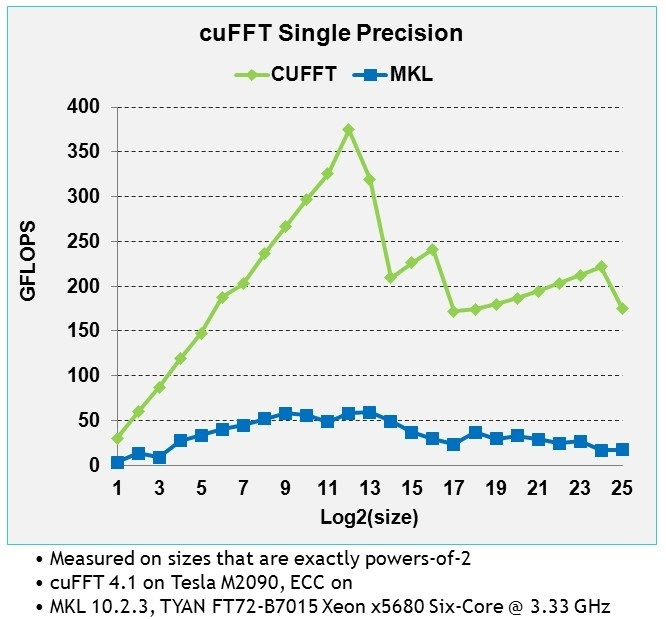
\includegraphics[width=3.5in]{cufftperformance.jpg}
\caption{A single-precision performance comparison between cuFFT and the Intel MKL Library \cite{nvidia:cufft}}
\label{fig:cufftmklperformance}
\end{figure}

\subsection{Non-Pipelined Approach}

To demonstrate the simplicity of achieving a speedup over a sequential implementation,
a somewhat trivial approach was implemented first. In this implementation, the algorithm
resembles the CPU version more closely than its pipelined counterpart. The signal data
is transferred in one large chunk from the host to the GPU, after which the FFT
is performed using the cuFFT API and the transmissions are detected using custom
CUDA kernels run in parallel. Considering this methods simplicity, it has a few notable
limitations. Firstly, we are limited to only computing on as much data that can be
held in GPU memory. Secondly, and perhaps more importantly, this method cannot be used
in realtime applications, as we are limited to performing the operations required
on a finite set of data. Dispite these limitations, this method is still able to 
achieve significant speedup over the sequential implementation.

\subsection{Pipelined Approach}

To hide the latency created by memory transfers across the PCIE bus, we can implement
a pipelining scheme. In this implementation, smaller pieces of data are transferred
incrementally to the device. This allows the GPU to begin work on some parts of 
the data as others are still being transferred over. If each of $N$ pipeline stages are
near equal in terms of time required to complete them, we can achieve a theoretical
speedup of $N$ over a non-pipelined solution. 

To do this, we split our algorithm up into four parts, or stages, to be pipelined.
The first stage transfers signal data from the host memory to the GPU. The second 
stage uses cuFFT to perform an FFT of size 4096 on the input data. The third stage performs
signal processing. More specifically, it calculates the complex modulus across
multiple FFT results to maximize GPU efficiency, as performing an operation on only
4096 elements will result in GPU memory latency, as many cores will be waiting for
memory access. The fourth and final stage detects transmissions by finding frequency
bins that exceed the signal threshold. If a frequency has exceeded the threshold it
will be noted in a bit array of size 4096. If the signal strength of a frequency that 
is active in the bit array has fallen below the threshold, the information about that
transmission will be noted in several device buffers for later transfer to the host.
In the current implementation, it was decided that due to the relatively small amount
of transmission data (in the range of 1KB) to be transfered back to the host, that
this action should not be pipelined. If re-implemented for realtime analysis of radio
signals, this process would have to be pipelined to allow transmissions to be
discovered while the program is running and processing signal data. The pipelined
process is illustrated in figure \ref{fig:pipeline}. 

\begin{figure}[ht!]
\centering
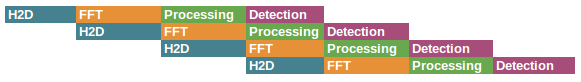
\includegraphics[width=3.5in]{pipeline.png}
\caption{A graphic illustrating a basic idea of a pipelined approach to the problem.}
\label{fig:pipeline}
\end{figure}

\section{Results}

The unpipelined implementation of the GPU program achieved a significant speedup
over its CPU counterpart, which peaked at around 53. As the number of elements
increased however, its speedup began to fall and stabilize at around 13 or 14. This
is due to two reasons. The first of which is a sub-optimized transmission recording
kernel. The kernel requires atomics to increment the number of transmissions detected,
as well as adding a new transmission to the transmission information buffers, which 
requires atomics to ensure that other threads do not overwrite eachothers 
transmissions. This kernel operation could be much further optimized to reduce this
performance bottleneck. Secondly, the lack of a dynamic signal threshold creates
many more transmissions in a high-noise section of the signal than a low-noise
section. Consequently, in these high noise sections that were encountered later
in the input file, many more transmissions were created and made the problem even
more pronounced. Implementing a dynamic signal threshold would likely solve this
issue. The speedup over the CPU version are illustrated in Figures \ref{fig:speedup}
and \ref{fig:speedupgraph}.

\begin{figure}[ht!]
\centering
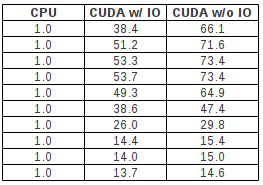
\includegraphics[width=3.5in]{speedup.png}
\caption{Table of GPU speedup over CPU implementation with and without I/O.}
\label{fig:speedup}
\end{figure}


\begin{figure}[ht!]
\centering
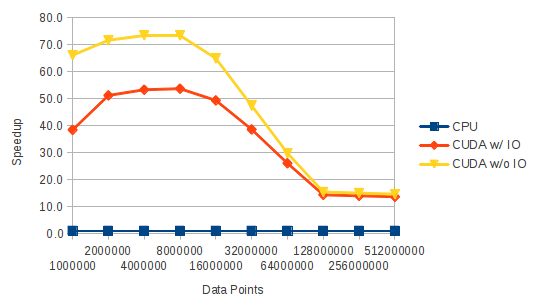
\includegraphics[width=3.5in]{speedupgraph.png}
\caption{Graph of GPU speedup over CPU implementation with and without I/O.}
\label{fig:speedupgraph}
\end{figure}

Unfortunately, the pipelined implementation was unable to be finished. There 
were a few different problems that were encountered that presented a significant
challenge for this implementation. First and foremost was a problem surrounding
the implementation of cuFFT. In the Cuda API, kernel calls are asynchronous
as well as asynchronous memory copies. Adding an asynchronous memory copy 
and a kernel call to a Cuda stream is an effective and relatively straightforward
way of implementing a GPU pipeline. For this to work, each of the calls in the
stream must be asynchronous, as the program running on the CPU must continue
to make calls to the Cuda API to manage the other streams. If a blocking call
is placed in the pipeline, the other streams will need to wait for that
particular operation to finish, which defeats the purpose of creating a 
pipeline in the first place since different steps cannot be executed at the 
same time. The cuFFT API call to execute a FFT is blocking for reasons
unbenounced to me. With the FFT being critical to the following steps
of the algorithm, we cannot avoid this outright. A possible solution would be to
execute the streams each in their separate thread, which would allow the
blocking calls to occur without disrupting the other streams. However when
calling the FFTs in separate threads, the result was runtime errors. The 
pipelined version also needs a more complicated transmission detection kernel.
Since there are several FFT's and processing being performed at different
times, we must traverse all of these to determine when and how long a
transmission has taken place.

\section{Conclusion}

In this paper, a method for performing signal processing and transmission
detection on a GPU was presented. Even with algorithmic deficiencies and
less-than-optimized kernels the program was able to achieve a 53 times
speedup. Used in a relatively low-noise environment, the method should
perform similar to test results. With additional work and testing, a
pipelined version could also be implemented. 

% An example of a floating figure using the graphicx package.
% Note that \label must occur AFTER (or within) \caption.
% For figures, \caption should occur after the \includegraphics.
% Note that IEEEtran v1.7 and later has special internal code that
% is designed to preserve the operation of \label within \caption
% even when the captionsoff option is in effect. However, because
% of issues like this, it may be the safest practice to put all your
% \label just after \caption rather than within \caption{}.
%
% Reminder: the "draftcls" or "draftclsnofoot", not "draft", class
% option should be used if it is desired that the figures are to be
% displayed while in draft mode.
%
%\begin{figure}[!t]
%\centering
%\includegraphics[width=2.5in]{myfigure}
% where an .eps filename suffix will be assumed under latex, 
% and a .pdf suffix will be assumed for pdflatex; or what has been declared
% via \DeclareGraphicsExtensions.
%\caption{Simulation Results}
%\label{fig_sim}
%\end{figure}

% Note that IEEE typically puts floats only at the top, even when this
% results in a large percentage of a column being occupied by floats.


% An example of a double column floating figure using two subfigures.
% (The subfig.sty package must be loaded for this to work.)
% The subfigure \label commands are set within each subfloat command, the
% \label for the overall figure must come after \caption.
% \hfil must be used as a separator to get equal spacing.
% The subfigure.sty package works much the same way, except \subfigure is
% used instead of \subfloat.
%
%\begin{figure*}[!t]
%\centerline{\subfloat[Case I]\includegraphics[width=2.5in]{subfigcase1}%
%\label{fig_first_case}}
%\hfil
%\subfloat[Case II]{\includegraphics[width=2.5in]{subfigcase2}%
%\label{fig_second_case}}}
%\caption{Simulation results}
%\label{fig_sim}
%\end{figure*}
%
% Note that often IEEE papers with subfigures do not employ subfigure
% captions (using the optional argument to \subfloat), but instead will
% reference/describe all of them (a), (b), etc., within the main caption.


% An example of a floating table. Note that, for IEEE style tables, the 
% \caption command should come BEFORE the table. Table text will default to
% \footnotesize as IEEE normally uses this smaller font for tables.
% The \label must come after \caption as always.
%
%\begin{table}[!t]
%% increase table row spacing, adjust to taste
%\renewcommand{\arraystretch}{1.3}
% if using array.sty, it might be a good idea to tweak the value of
% \extrarowheight as needed to properly center the text within the cells
%\caption{An Example of a Table}
%\label{table_example}
%\centering
%% Some packages, such as MDW tools, offer better commands for making tables
%% than the plain LaTeX2e tabular which is used here.
%\begin{tabular}{|c||c|}
%\hline
%One & Two\\
%\hline
%Three & Four\\
%\hline
%\end{tabular}
%\end{table}


% Note that IEEE does not put floats in the very first column - or typically
% anywhere on the first page for that matter. Also, in-text middle ("here")
% positioning is not used. Most IEEE journals/conferences use top floats
% exclusively. Note that, LaTeX2e, unlike IEEE journals/conferences, places
% footnotes above bottom floats. This can be corrected via the \fnbelowfloat
% command of the stfloats package.

% conference papers do not normally have an appendix


% use section* for acknowledgement
\section*{Acknowledgment}


The authors would like to thank...

\cite{IEEEhowto:IEEEtranpage}



% trigger a \newpage just before the given reference
% number - used to balance the columns on the last page
% adjust value as needed - may need to be readjusted if
% the document is modified later
%\IEEEtriggeratref{8}
% The "triggered" command can be changed if desired:
%\IEEEtriggercmd{\enlargethispage{-5in}}

% references section

% can use a bibliography generated by BibTeX as a .bbl file
% BibTeX documentation can be easily obtained at:
% http://www.ctan.org/tex-archive/biblio/bibtex/contrib/doc/
% The IEEEtran BibTeX style support page is at:
% http://www.michaelshell.org/tex/ieeetran/bibtex/
%\bibliographystyle{IEEEtran}
% argument is your BibTeX string definitions and bibliography database(s)
%\bibliography{IEEEabrv,../bib/paper}
%
% <OR> manually copy in the resultant .bbl file
% set second argument of \begin to the number of references
% (used to reserve space for the reference number labels box)
%\begin{thebibliography}{1}
%
%\bibitem{IEEEhowto:kopka}
%H.~Kopka and P.~W. Daly, \emph{A Guide to \LaTeX}, 3rd~ed.\hskip 1em plus
%  0.5em minus 0.4em\relax Harlow, England: Addison-Wesley, 1999.
%
%\end{thebibliography}

\bibliographystyle{IEEEtran}	% (uses file "plain.bst")
\bibliography{refs}		% expects file "myrefs.bib"



% that's all folks
\end{document}


